% Hauptinhalt der Arbeit
\section{Einleitung: Die Vitalzeichen einer Plattform}

Eine Frage wird abgeschickt, die Oberfläche wirkt kurz wie eingefroren, und irgendwo im Hintergrund beginnt eine Kette aus Diensten zu arbeiten. Kommt die Antwort in Sekunden -- oder bleibt der Nutzer vor einem Ladeindikator hängen? In cloud-nativen Systemen entscheidet sich die Qualität einer Anwendung nicht nur im Quellcode, sondern im Betrieb: in Lastspitzen, in Randfällen, an Schnittstellen zu externen Diensten. Genau dort steigt die Komplexität, weil verteilte Architekturen zwar flexibel skalieren und Komponenten unabhängig weiterentwickeln lassen, zugleich aber die Überwachung und Fehlersuche spürbar erschweren \cite{faseeha2025observability,sakinala2025observability}. Besonders Microservices erzeugen Fehlerbilder, deren Ursache nicht mehr eindeutig „einem“ Baustein zugeordnet werden kann, weil Abhängigkeiten und Nebenwirkungen über Service-Grenzen hinweg wirken \cite{fischer2024microservice}.

Hier setzt Observability an: Nicht als neues Buzzword, sondern als Versuch, den inneren Zustand eines Systems aus seinen messbaren „Ausgaben“ zu verstehen. Dazu werden Metriken, Logs und Traces gemeinsam betrachtet, um Verhalten, Fehler und Leistungsmerkmale in Beziehung zu setzen \cite{sridharan2018distributed,faseeha2025observability}. Empirische Arbeiten aus dem Umfeld cloud-nativer Anwendungen berichten, dass strukturierte Observability-Praktiken die Incident-Analyse unterstützen und Reaktionszeiten verkürzen können \cite{giamattei2024monitoring,sakinala2025observability}. Die zentrale Frage lautet also: Welche „Vitalzeichen“ zeigen zuverlässig, ob ein Dienst gesund ist -- und welche Daten helfen tatsächlich, wenn es kritisch wird?

Diese Arbeit trägt den Titel: \textit{Die Vitalzeichen einer Plattform: Wie man mit Observability den Gesundheitszustand von frag.jetzt überwacht}. Im Mittelpunkt steht die Open-Source-Plattform \textit{frag.jetzt}, deren Kernwert im produktiven Betrieb davon abhängt, dass Nutzerfragen entlang eines verteilten Anfragepfads schnell, korrekt und nachvollziehbar beantwortet werden \cite{fragjetztRepo}. Trotz einer soliden Entwicklungs- und Deployment-Infrastruktur fehlt derzeit ein durchgängiges Observability-Konzept, das Metriken, Logs, Traces und Alarmierung konsistent entlang dieser End-to-End-Kette verbindet \cite{fragjetztRepo,giamattei2024monitoring}. Dadurch bleiben Zusammenhänge zwischen Nutzererlebnis, Backend-Verarbeitung und externen Abhängigkeiten nur eingeschränkt sichtbar.

\begin{figure}[H]
\centering
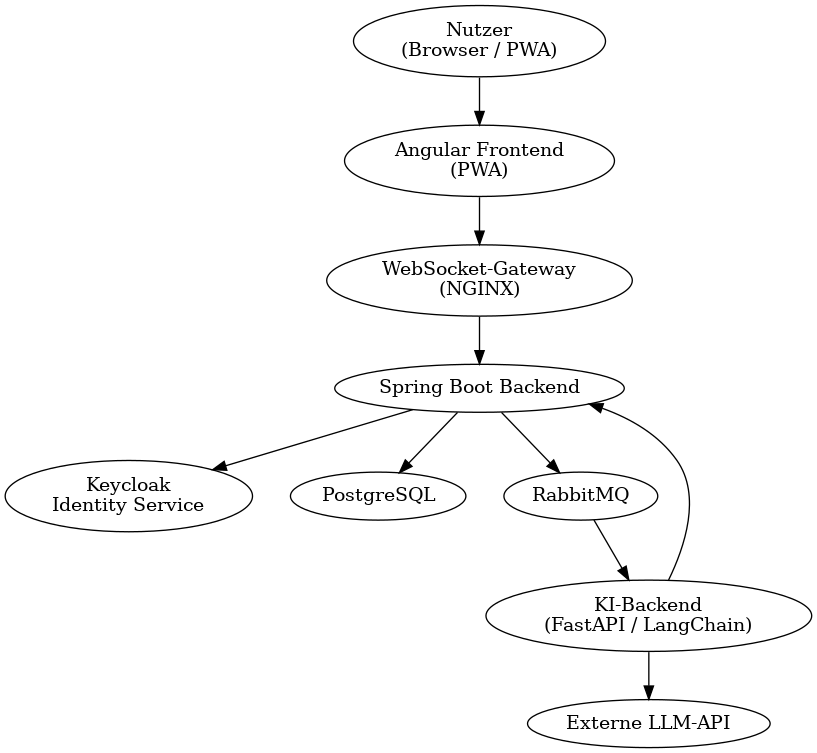
\includegraphics[width=0.92\columnwidth]{images/fragjetzt-request-path.png}
\caption{Vereinfachter Anfragepfad bei \textit{frag.jetzt}: Von der Nutzerfrage bis zur Antwort über mehrere Komponenten hinweg. Quelle: Eigene Darstellung in Anlehnung an die Architekturübersicht im Projekt-Repository \cite{fragjetztRepo}.}
\label{fig:request-path}
\end{figure}

\subsection{Warum gerade jetzt? Drei Beobachtungen aus dem Forschungsstand}

Erstens: Die Literatur beschreibt wiederkehrend, dass klassische Monitoring-Ansätze in dynamischen, verteilten Umgebungen an Grenzen stoßen, weil sie vor allem bekannte Fehlerzustände mit statischen Schwellenwerten überwachen, aber bei unbekannten Störungen wenig Hilfestellung liefern \cite{sridharan2018distributed,sakinala2025observability}. Zweitens: Moderne Observability wird in Studien als Kombination mehrerer Telemetriearten verstanden -- erst ihr Zusammenspiel ermöglicht robuste Ursachenanalyse \cite{abieba2025advanced,sakinala2025observability}. Drittens: Alarmierung gilt als besondere Schwachstelle, weil zu viele Fehlalarme („Alarmmüdigkeit“) operative Entscheidungen verschlechtern; daher werden Priorisierung und datenbasierte Verfahren zur Reduktion irrelevanter Alarme als Forschungsschwerpunkte diskutiert \cite{jalalvand2024alert}.

Damit rückt eine pragmatische Leitfrage nach vorn: Welche Signale helfen im Alltag der Plattform wirklich -- für DevOps, Entwicklung und Produktverantwortliche gleichermaßen?

\section{Vier Golden Signals als Vitalzeichen: hilfreich, aber nicht selbsterklärend}

Ein oft genutzter Startpunkt sind die \textit{Four Golden Signals} aus Googles Site Reliability Engineering: \textit{Latency}, \textit{Traffic}, \textit{Errors} und \textit{Saturation} \cite{ewaschukMonitoringDistributedSystems}. Sie wirken wie ein medizinischer Schnellcheck: Sie liefern Symptome, aber noch keine Diagnose. Genau diese Stärke macht sie so attraktiv, denn sie sind universell genug, um auf nahezu jeden nutzerorientierten Dienst angewandt zu werden \cite{ewaschukMonitoringDistributedSystems}. Gleichzeitig wird betont, dass ihre Wirksamkeit davon abhängt, wie sie in Alarmierung, Entscheidungsprozesse und betriebliche Abläufe eingebettet werden \cite{ewaschukMonitoringDistributedSystems}.

\begin{itemize}
  \item \textbf{Latenz:} Wie lange dauert es, bis eine Anfrage bearbeitet ist? Hohe oder schwankende Zeiten deuten auf Engpässe hin \cite{ewaschukMonitoringDistributedSystems}.
  \item \textbf{Traffic:} Wie viel Last trifft auf einen Dienst? Einbrüche können ebenso verdächtig sein wie Spitzen \cite{ewaschukMonitoringDistributedSystems}.
  \item \textbf{Fehler:} Wie viele Anfragen schlagen fehl -- technisch oder funktional? \cite{ewaschukMonitoringDistributedSystems}
  \item \textbf{Sättigung:} Wie ausgelastet sind limitierende Ressourcen wie CPU, Speicher, I/O oder Warteschlangen? \cite{ewaschukMonitoringDistributedSystems}
\end{itemize}

Die entscheidende Zuspitzung lautet: Ein korrekt gemessener Wert ist noch keine handlungsrelevante Information. Ein Alarm, der niemandem sagt, \textit{wer} betroffen ist, \textit{wie stark} der Schaden ausfällt und \textit{welche} nächsten Schritte plausibel sind, bleibt nur Lärm \cite{jalalvand2024alert}.

\section{Der Patient: \textit{frag.jetzt} als verteiltes System mit kritischem Pfad}

\textit{frag.jetzt} ist eine Cloud-native Q\&A-Plattform, die interaktive Fragerunden unterstützt und zusätzlich KI-gestützte Assistenzfunktionen integriert \cite{fragjetztRepo}. Der zentrale Pfad ist aus Nutzersicht simpel: \textit{Frage stellen} $\rightarrow$ \textit{Antwort erhalten}. Technisch wird dieser Ablauf jedoch über mehrere Komponenten umgesetzt, darunter ein Angular-Frontend (SPA/PWA), ein WebSocket-Gateway (NGINX), ein Spring-Boot-Backend, Authentifizierung über Keycloak, Persistenz in PostgreSQL sowie ein KI-Backend (u.\,a.\ FastAPI/Langchain) mit externen LLM-Abhängigkeiten; asynchrone Entkopplung kann über RabbitMQ erfolgen \cite{fragjetztRepo}. Jeder zusätzliche Hop ist ein potenzieller Latenzpunkt, jeder externe Dienst eine Fehlerquelle, und jede Warteschlange kann sich unbemerkt füllen -- bis es für Nutzer sichtbar wird.

\subsection{Welche Fragen muss ein Betriebsteam in Sekunden beantworten können?}

Statt Telemetrie als Selbstzweck zu sammeln, beginnt Observability mit Fragen. Für \textit{frag.jetzt} drängen sich insbesondere diese Fragen auf:

\begin{itemize}
  \item \textbf{Nutzererlebnis:} Wird die Antwort schnell genug sichtbar -- oder entsteht „gefühlte“ Langsamkeit im Frontend?
  \item \textbf{Fehlerlokalisierung:} Liegt das Problem im Spring-Boot-Backend, in der Datenbank, im Auth-Flow oder in der externen KI-API?
  \item \textbf{Abhängigkeiten:} Verursacht eine schwankende externe KI-Latenz Kaskadeneffekte, etwa Stau in Queues oder erschöpfte Verbindungspools?
  \item \textbf{Priorisierung:} Betrifft die Störung wenige Anfragen oder das Kernfeature? Ist sofortiges Eingreifen nötig?
\end{itemize}

Gerade diese Verbindung aus Technik und Nutzungskontext wird in der Literatur als Hebel beschrieben, um Observability im Betrieb wirksam zu machen \cite{abieba2025advanced,giamattei2024monitoring}.

\section{Werkzeuge als Diagnosegeräte: Metriken, Logs, Traces -- und der Streit um den Stack}

In der Praxis existiert kein „ein“ Observability-Tool. Vielmehr werden spezialisierte Bausteine kombiniert: Metriken liefern Trends und Grenzwerte, Logs zeigen Ereignisdetails, Traces rekonstruieren den Weg einzelner Anfragen durch verteilte Systeme \cite{abieba2025advanced,sakinala2025observability}. Distributed Tracing wird dabei besonders für Microservices als essenziell beschrieben, weil es Latenzengpässe und Abhängigkeiten entlang des gesamten Anfragepfads sichtbar macht \cite{albuquerque2025tracing}.

Für die Werkzeugauswahl stehen in Open-Source-Ökosystemen mehrere etablierte Optionen bereit:

\begin{itemize}
  \item \textbf{Prometheus} zur Erfassung und Abfrage zeitbasierter Metriken (inkl.\ regelbasiertem Alerting) \cite{banerjee2024comparative}.
  \item \textbf{Grafana} zur Visualisierung und Korrelation verschiedener Datenquellen \cite{giamattei2024monitoring}.
  \item \textbf{Elastic Stack (ELK)} als verbreitete Lösung für zentrale Log-Aggregation und Analyse \cite{banerjee2024comparative}.
  \item \textbf{Jaeger} für Distributed Tracing und End-to-End-Latenzanalyse \cite{albuquerque2025tracing}.
  \item \textbf{OpenTelemetry} als herstellerneutraler Standard zur Instrumentierung für Metriken, Logs und Traces \cite{albuquerque2025tracing}.
\end{itemize}

Vergleichsstudien diskutieren diese Toolklassen entlang von Kriterien wie Telemetrieabdeckung, Integrationsfähigkeit, Skalierbarkeit und Betriebsaufwand \cite{giamattei2024monitoring,banerjee2024comparative}. Daraus ergibt sich eine praktische, aber forschungsnahe Auswahlfrage: Welche Kombination passt am besten zu den Anforderungen und Ressourcen von \textit{frag.jetzt}? \\

\captionsetup{type=table}
\begin{minipage}{\columnwidth}
\centering
\footnotesize
\setlength{\tabcolsep}{3.5pt}
\renewcommand{\arraystretch}{1.2}
\begin{tabularx}{\columnwidth}{@{}>{\RaggedRight\arraybackslash}p{0.36\columnwidth} >{\RaggedRight\arraybackslash}X@{}}
\toprule
\textbf{Entscheidungsfrage} & \textbf{Warum sie zählt} \\
\midrule
Metriken-first oder Logs-first? & Metriken zeigen Trends, Logs liefern Details — beeinflusst Kosten und Diagnosezeit. \cite{abieba2025advanced} \\
Tracing-Pflicht? & Ohne End-to-End-Traces bleiben Engpässe und Abhängigkeiten in Microservices schwer greifbar. \cite{albuquerque2025tracing} \\
Instrumentierung mit Standard? & OpenTelemetry entkoppelt Erfassung vom Backend und reduziert Risiko eines Vendor Lock-ins. \cite{albuquerque2025tracing} \\
\bottomrule
\end{tabularx}
\caption{Leitfragen zur Stack-Auswahl für Observability. Quelle: Eigene Darstellung auf Basis der Literatur \cite{abieba2025advanced,albuquerque2025tracing,giamattei2024monitoring}.}
\label{tab:stack-questions}
\end{minipage}

\section{Forschungsfragen: Von Vitalzeichen zu Entscheidungen}

Aus Problemstellung, Architektur und Forschungsstand leiten sich drei Forschungsfragen ab:

\begin{enumerate}
\item Wie können die Four Golden Signals für die spezifischen Services von \textit{frag.jetzt} (PWA-Frontend, Spring Boot Backend, PostgreSQL, KI-Services) konkret definiert und instrumentiert werden? \cite{ewaschukMonitoringDistributedSystems,faseeha2025observability}
\item Welche Observability-Stack-Kombination (Prometheus/Grafana, ELK Stack, Jaeger) ist am besten geeignet für die Monitoring-Anforderungen von \textit{frag.jetzt}? \cite{giamattei2024monitoring,banerjee2024comparative}
\item Wie kann ein intelligentes Alert-System entwickelt werden, das False Positives minimiert und handlungsorientierte Einblicke für verschiedene Rollen (DevOps, Entwicklung, Product Owner) bereitstellt? \cite{jalalvand2024alert}
\end{enumerate}

\section{Methodik als Storyline: Sechs Schritte vom Symptom zur Therapie}

Die Arbeit folgt einem artefaktorientierten Forschungsdesign mit konzeptionellem und prototypischem Schwerpunkt. Statt jeden Baustein bis ins letzte Detail zu erklären, wird eine nachvollziehbare „Diagnosekette“ aufgebaut -- von der Definition der Vitalzeichen bis zu Runbooks, die im Incident-Fall konkrete Schritte liefern.

\subsection{Schritt 1: Golden Signals pro Komponente konkretisieren}

Die Golden Signals werden für jedes Teilsystem so interpretiert, dass sie sowohl aus Technik- als auch aus Nutzungsperspektive verständlich sind \cite{ewaschukMonitoringDistributedSystems}. Für ein PWA-Frontend kann „Latenz“ etwa als wahrgenommene Antwortzeit erscheinen, während im Backend zusätzliche Perspektiven (API-Latenz, Queue-Wartezeiten, Datenbank-Response) relevant werden \cite{faseeha2025observability}.

\subsection{Schritt 2: Tool-Stacks vergleichen und begründet auswählen}

Da eine vollständige praktische Erprobung aller Werkzeuge im Rahmen der Arbeit unrealistisch ist, wird der Vergleich primär theoretisch-konzeptionell durchgeführt. Bewertet werden u.\,a.\ Telemetrieabdeckung, Integrationsfähigkeit, Betriebsaufwand und Reifegrad \cite{giamattei2024monitoring,banerjee2024comparative}. Ergebnis ist eine begründete Stack-Empfehlung für \textit{frag.jetzt}.

\subsection{Schritt 3: Instrumentierung entlang des Anfragepfads}

OpenTelemetry dient als einheitliche Instrumentierungsschicht, um Metriken, Logs und Traces konsistent zu erfassen und korrelierbar zu machen \cite{albuquerque2025tracing}. Entscheidend ist dabei nicht die Menge an Daten, sondern die Fähigkeit, eine Nutzeranfrage über Systemgrenzen hinweg wiederzufinden.

\subsection{Schritt 4: Dashboards, die Rollen statt Datenquellen abbilden}

Dashboards werden rollenbasiert konzipiert, damit nicht jede Zielgruppe dieselben Rohdaten interpretieren muss. Während DevOps eine schnelle Systemübersicht benötigt, interessiert die Entwicklung oft der Drilldown bis zum Trace, und Product Owner benötigen eine Sicht auf Nutzerwirkung und Priorität \cite{giamattei2024monitoring}.

\subsection{Schritt 5: Alarmierung, die Relevanz und Dringlichkeit kennt}

Ein Alerting-Ansatz wird entworfen, der sich an den Golden Signals orientiert und zugleich Mechanismen zur Reduktion irrelevanter Alarme berücksichtigt, etwa Aggregation mehrerer Signale, zeitliche Glättung und einfache Anomalieerkennung \cite{jalalvand2024alert}. Ziel ist eine Alarmierung, die nicht nur „etwas ist anders“ ruft, sondern beantwortet: \textit{Ist Handeln nötig, wen betrifft es, und was ist der nächste sinnvolle Schritt?}

\subsection{Schritt 6: Runbooks als operationalisierte Erfahrung}

Runbooks werden für wiederkehrende Incident-Szenarien erstellt und verknüpfen Alerts mit Diagnose- und Handlungsanweisungen. Damit wird Wissen aus der Telemetrie in operative Routine überführt, was in Observability-Ansätzen als wichtiger Baustein zur Verkürzung der Reaktionszeit gilt \cite{giamattei2024monitoring,sakinala2025observability}.

\section{Ergebnisartefakte: Was am Ende „in der Hand“ liegt}

Aus den Schritten ergeben sich vier geplante Artefakte:
\begin{enumerate}
  \item ein wissenschaftlicher Bericht zur Strategie, Toolauswahl und Alarmierungskonzeption,
  \item eine lauffähige Observability-Plattform (z.\,B.\ Prometheus/Grafana) für \textit{frag.jetzt},
  \item rollenbasierte Dashboards,
  \item exemplarische Runbooks für typische Incident-Situationen.
\end{enumerate}

\section{Fazit und Ausblick: Wenn Vitalzeichen zu Vertrauen werden}

Observability ist dann gelungen, wenn aus Telemetrie Vertrauen entsteht: Vertrauen, dass Nutzer nicht im Dunkeln warten, dass Fehler nicht nur entdeckt, sondern erklärt werden können, und dass Betriebsteams handlungsfähig bleiben, auch wenn externe Abhängigkeiten schwanken. Die Literatur zeigt, dass gerade in cloud-nativen Systemen strukturierte Observability-Praktiken die Analyse von Störungen unterstützen und operative Reaktionszeiten verkürzen können \cite{giamattei2024monitoring,sakinala2025observability}. Für \textit{frag.jetzt} wird dieser Gedanke in eine konkrete Strategie übersetzt, die Golden Signals als Einstieg nutzt, aber durch Kontext, Tracing-Korrelation, rollenbasierte Sichten und priorisierte Alarmierung in Richtung betrieblicher Nutzbarkeit erweitert \cite{ewaschukMonitoringDistributedSystems,albuquerque2025tracing,jalalvand2024alert}.

Im Ausblick bieten sich insbesondere SLO-basierte Steuerung und eine schrittweise Reifegradsteigerung an, um technische Symptome noch konsequenter mit Nutzerwirkung zu verbinden \cite{ewaschukMonitoringDistributedSystems,giamattei2024monitoring}. Damit würden aus vier Vitalzeichen nicht nur Messwerte, sondern ein belastbarer Gesundheitscheck für eine Plattform, die von Interaktion lebt.


\section*{Abkürzungsverzeichnis}

\begin{tabular}{p{1.5cm} p{11cm}}
API        & Application Programming Interface \\
CI/CD      & Continuous Integration /\\
           & Continuous Deployment \\
CPU        & Central Processing Unit \\
ELK        & Elasticsearch, Logstash, Kibana \\
HTTP       & Hypertext Transfer Protocol \\
HTTPS     & Hypertext Transfer Protocol Secure \\
KI         & Künstliche Intelligenz \\
NLP        & Natural Language Processing \\
OTel      & OpenTelemetry \\
PWA       & Progressive Web App \\
Q\&A      & Question and Answer \\
REST      & Representational State Transfer \\
% SLA       & Service Level Agreement \\
% SLI       & Service Level Indicator \\
SLO       & Service Level Objective \\
SPA       & Single-Page Application \\
SRE       & Site Reliability Engineering \\
UI        & User Interface \\
\end{tabular}

% \begin{acronym}[CI/CD]
%   \acro{API}{Application Programming Interface}
%   \acro{CI/CD}{Continuous Integration / Continuous Deployment}
%   \acro{CPU}{Central Processing Unit}
%   \acro{ELK}{Elasticsearch, Logstash, Kibana}
%   \acro{HTTP}{Hypertext Transfer Protocol}
%   \acro{HTTPS}{Hypertext Transfer Protocol Secure}
%   \acro{KI}{Künstliche Intelligenz}
%   \acro{NLP}{Natural Language Processing}
%   \acro{OTel}{OpenTelemetry}
%   \acro{PWA}{Progressive Web App}
%   \acro{Q&A}{Question and Answer}
%   \acro{REST}{Representational State Transfer}
%   \acro{SLA}{Service Level Agreement}
%   \acro{SLI}{Service Level Indicator}
%   \acro{SLO}{Service Level Objective}
%   \acro{SPA}{Single-Page Application}
%   \acro{SRE}{Site Reliability Engineering}
%   \acro{UI}{User Interface}
% \end{acronym}

% \section*{Glossar}

% \begin{description}
%   \item[Agent:] Ein KI-System, das eigenständig Ziele verfolgt, Pläne erstellt und Werkzeuge nutzt – im Gegensatz zu passiven Chatbots.
  
%   \item[Chain-of-Thought:] Technik, bei der ein Sprachmodell angewiesen wird, seinen Denkprozess explizit zu formulieren, was zu besseren Ergebnissen führt.
  
%   \item[Halluzination:] Das Phänomen, dass Sprachmodelle plausibel klingende, aber faktisch falsche Informationen generieren.
  
%   \item[LLM (Large Language Model):] Großes Sprachmodell wie GPT-4 oder Claude, das auf riesigen Textmengen trainiert wurde.
  
%   \item[Prompt Injection:] Angriffstechnik, bei der schädliche Anweisungen in Eingabedaten versteckt werden, um ein KI-System zu manipulieren.
  
%   \item[RAG (Retrieval-Augmented Generation):] Methode, bei der ein Sprachmodell vor der Antwortgenerierung relevante Informationen aus einer Datenbank abruft.
  
%   \item[ReAct:] \enquote{Reasoning and Acting} – Methodik, bei der Agenten explizit zwischen Denken und Handeln alternieren.
  
%   \item[Sandbox:] Isolierte Ausführungsumgebung, die verhindert, dass Code das umgebende System beeinflusst.
  
%   \item[Token:] Grundeinheit der Textverarbeitung in Sprachmodellen – grob entspricht ein Token 0,75 Wörtern.
  
%   \item[Vektor-Datenbank:] Spezielle Datenbank zur Speicherung und schnellen Suche von semantisch ähnlichen Texten oder Code.
% \end{description}
